\begin{frame}{Starting Point: The NSAK Framework}
    \framesubtitle{Established in the predecessor project (Project 2)}

    \begin{columns}[T,onlytextwidth]
        \begin{column}{0.5\textwidth}
            \vspace*{0.8cm}
            \textbf{A modular, open-source network security}\\\textbf{framework}

            \vspace{0.6em}
            Built around four reusable resource types:
            \vspace{0.4em}
            \begin{itemize}
                \item[\faServer] \textbf{Device} \textit{\scriptsize execution host at a network position}
                \item[\faNetworkWired] \textbf{Environment} \textit{\scriptsize target network topology}
                \item[\faLayerGroup] \textbf{Scenario} \textit{\scriptsize a red/blue team use case}
                \item[\faCogs] \textbf{Drill} \textit{\scriptsize reusable building block}
            \end{itemize}
        \end{column}

        \begin{column}{0.5\textwidth}
            \centering
            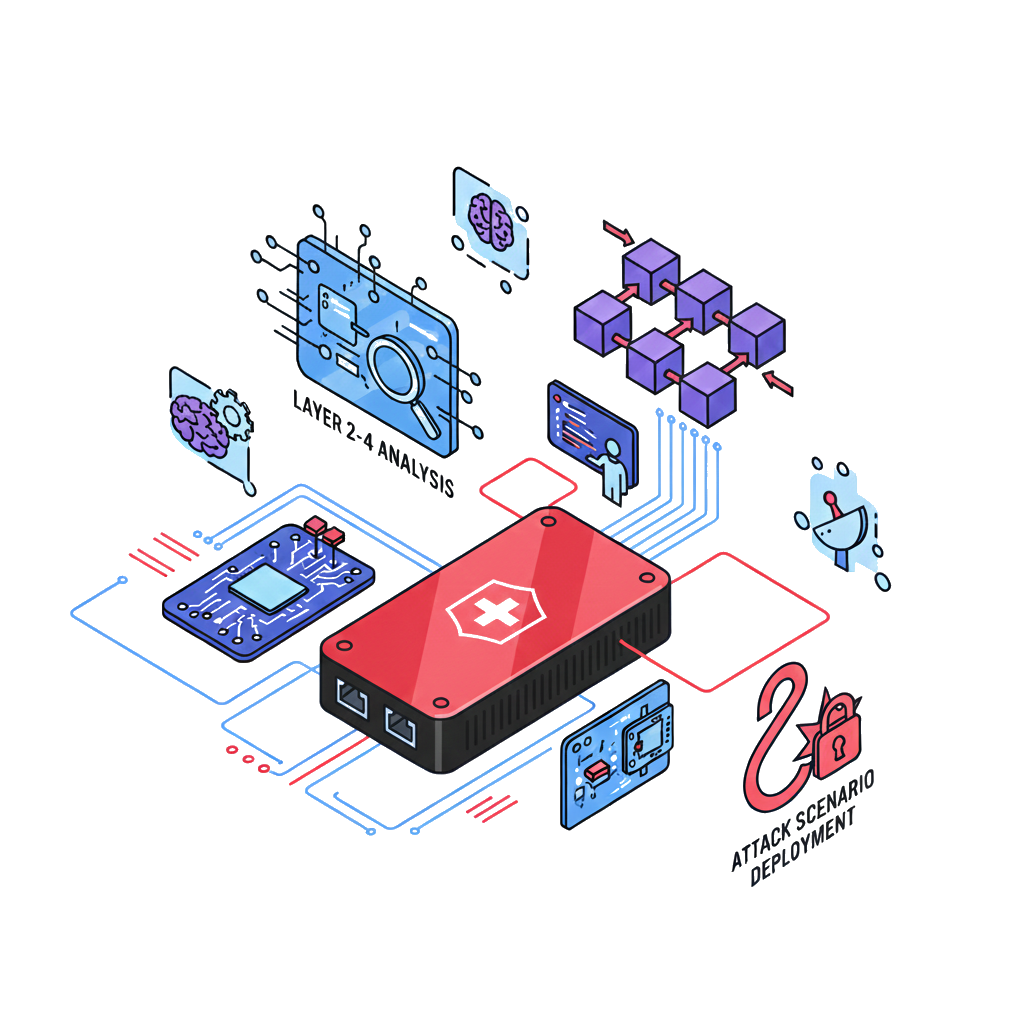
\includegraphics[width=0.9\linewidth]{assets/swiss-army-nsak-transparent}
        \end{column}
    \end{columns}
\end{frame}
\begin{frame}
    \begin{columns}[T,onlytextwidth]
        \begin{column}{0.5\textwidth}
            \begin{figure}
                \centering
                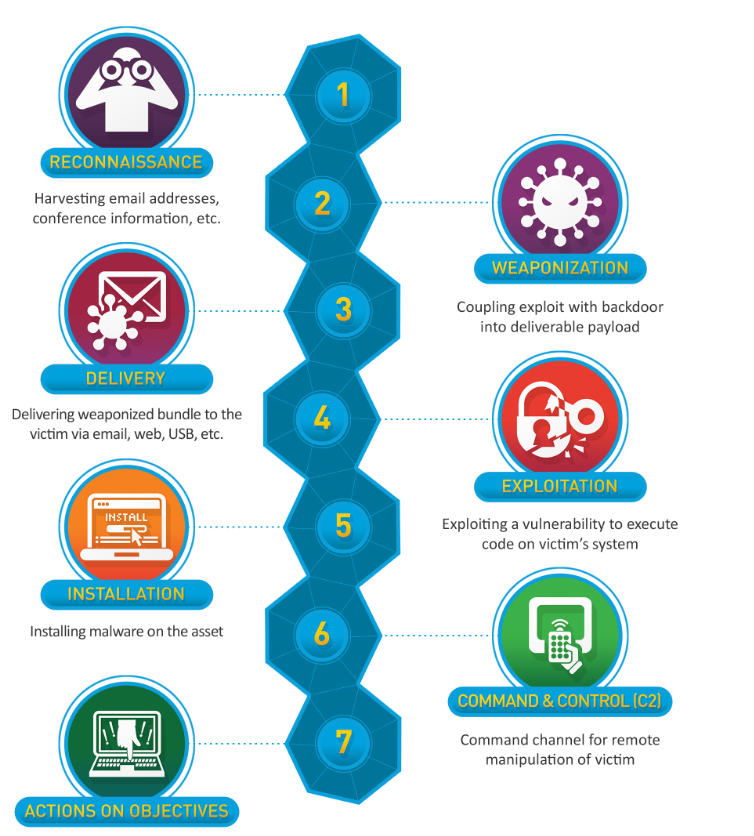
\includegraphics[width=0.9\linewidth]{assets/cyber-kill-chain}
                \label{fig:cyber-kill-chain}
            \end{figure}
        \end{column}

        \begin{column}{0.5\textwidth}
            \vspace*{1.5cm}

            \begin{itemize}
                \item Gather baseline data
                \item Detect
                \item Alert
                \item Investigate
                \item Plan a response
                \item Execute
            \end{itemize}
        \end{column}
    \end{columns}
\end{frame}
\begin{frame}
\begin{figure}
    \centering
    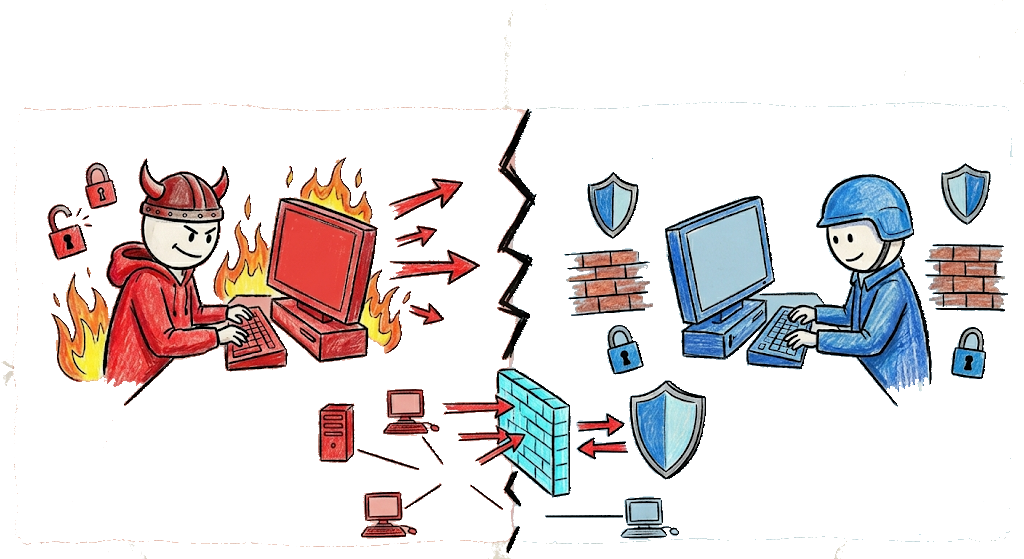
\includegraphics[width=0.8\linewidth]{assets/red-and-blue-v2-transparent}
    \caption{Red and Blue Team}
    \label{fig:red-and-blue-transparent}
\end{figure}
\end{frame}




\begin{frame}{Reconnaissance}
    \framesubtitle{The first stage of the cyber kill chain}

    \begin{columns}[T,onlytextwidth]
        \begin{column}{0.5\textwidth}
            \centering
            
\includegraphics[width=\linewidth]{assets/reconnaissance}
            \label{fig:reconnaissance}
        \end{column}

        \begin{column}{0.5\textwidth}
            \vspace{1cm}
            \small
            Gathering information about a target network \emph{before} any attack~--~it builds the
            map every later stage relies on, and is the focus of this thesis.
            \vspace{0.3em}
            \begin{itemize}
                \item[\faSearch] \textbf{Host discovery} \textit{\scriptsize which systems are reachable on the network}
                \item[\faNetworkWired] \textbf{Service \& port enumeration} \textit{\scriptsize what is running and exposed}
                \item[\faBug] \textbf{Characterization} \textit{\scriptsize OS, versions and vulnerability indicators}
            \end{itemize}
        \end{column}
    \end{columns}
\end{frame}

\begin{frame}{Hypothesis and Research Questions}
    \framesubtitle{From static scenarios to agentic AI}
    \uncover<1->{
        \begin{block}{Hypothesis}

            \small
            Integrating \textbf{agentic AI} into NSAK improves \textbf{adaptability, flexibility} and
            \textbf{automation} over static scenarios, while \textbf{lowering the operator's required expertise}
            to interpret results and plan follow-up steps.

        \end{block}
    }

    \vspace{0.4em}
    \uncover<2->{
        \begin{itemize}
            \item[\textbf{RQ1}] How does an agentic AI scenario perform \textbf{compared to a static reference} scenario in network reconnaissance?
            \item[\textbf{RQ2}] To what extent can agentic AI \textbf{support operators} during interactive reconnaissance?
            \item[\textbf{RQ3}] To what extent is the implementation \textbf{suitable for real-world} deployment?
        \end{itemize}
    }
\end{frame}
\begin{frame}{Project Goals}
    \framesubtitle{Order of implementation: Must $\rightarrow$ Should $\rightarrow$ Could}

    \centering
    \begin{tikzpicture}[font=\scriptsize,
        dot/.style={circle,fill,inner sep=2.2pt},
        phase/.style={font=\footnotesize\bfseries},
        goals/.style={anchor=north,align=left,text width=3.5cm}]

        % --- timeline axis ---
        \draw[->,line width=1.4pt,gray!70] (-5.6,0) -- (5.8,0);

        % ===== MUST =====
        \begin{scope}[visible on=<1->]
            \draw[red!75!black] (-4,0) -- (-4,-0.55);
            \node[dot,red!75!black] at (-4,0) {};
            \node[phase,red!75!black,above=2pt] at (-4,0.05) {Must};
            \node[goals] at (-3.5,-0.6) {
                Compare Frameworks\\
                AI Integration Research\\
                Configuration Management\\
                AI Scenarios\\
                Reproducible Test Env.\\
                Red Team Reconnaissance\\
                AI Scenario Evaluation\\
                AI vs.\ Engineered (Red)};
        \end{scope}

        % ===== SHOULD =====
        \begin{scope}[visible on=<2->]
            \draw[orange] (0.2,0) -- (0.2,-0.55);
            \node[dot,orange] at (0.2,0) {};
            \node[phase,orange,above=2pt] at (0.2,0.05) {Should};
            \node[goals] at (0.6,-0.6) {
                Blue Team Intrusion Detection\\
                AI vs.\ Engineered (Blue)};
        \end{scope}

        % ===== COULD =====
        \begin{scope}[visible on=<3->]
            \draw[gray!60] (4.2,0) -- (4.2,-0.55);
            \node[dot,gray!60] at (4.2,0) {};
            \node[phase,gray!60!black,above=2pt] at (4.2,0.05) {Could};
            \node[goals] at (5.2,-0.6) {
                REST API\\
                MCP Server\\
                Web GUI};
        \end{scope}
    \end{tikzpicture}
\end{frame}
